\chapter{Graph colouring}
\section*{Avoiding clashes}
A proper vertex-colouring assigns colours to vertices so adjacent vertices receive different colours. The smallest number of colours needed is the chromatic number, written $\chiG(G)$. In a scheduling model, colours may represent time slots; in a map model, they may represent regions.

\begin{figure}[htbp]
\centering
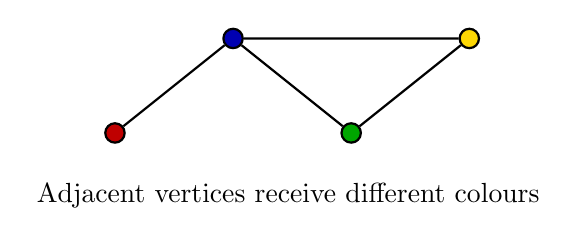
\begin{tikzpicture}[thick,vertex/.style={circle,draw=black,inner sep=0pt,minimum size=7pt}]
\node[vertex,fill=red!75!black] (a) at (0,0) {};
\node[vertex,fill=blue!70!black] (b) at (1.5,1.2) {};
\node[vertex,fill=green!65!black] (c) at (3,0) {};
\node[vertex,fill=yellow!75!orange] (d) at (4.5,1.2) {};
\draw (a)--(b)--(c)--(d) (b)--(d);
\node[draw=none,rectangle,fill=white] at (2.2,-0.8) {Adjacent vertices receive different colours};
\end{tikzpicture}
\caption{A proper colouring assigns different colours to the endpoints of every edge.}
\end{figure}

\begin{theorem}
A graph is bipartite if and only if it is 2-colourable (where a graph with no edges needs at most one colour).
\end{theorem}
\begin{proof}
If a graph is bipartite, give one colour to each vertex class. Conversely, the two colour classes of any proper 2-colouring contain no internal edges, so they form a bipartition.
\end{proof}

A greedy colouring processes vertices in some order, giving each the first colour not used by an already-coloured neighbour. If the maximum degree is $\Delta$, at most $\Delta$ colours are forbidden at any step, so $\Delta+1$ colours always suffice. The chosen order can make a big difference to how many colours greedy actually uses.

\begin{example}
For a triangle, greedy colouring requires three colours whatever the order, so $\chiG(K_3)=3$. For a path with at least one edge, alternating two colours works, and one cannot suffice, so its chromatic number is 2.
\end{example}

\begin{theorem}[\Challenge{} Five-colour theorem]
Every finite simple planar graph can be properly coloured with at most five colours.
\end{theorem}
\begin{proof}
We use induction on the number of vertices. The result is immediate for graphs with at most five vertices. For a planar graph with $n\geq 6$ vertices, Euler's planar edge bound implies that some vertex $v$ has degree at most 5: otherwise the degree sum would be at least $6n$, while $2m\leq 6n-12$. Remove $v$ and, by induction, colour the remaining graph with five colours. If $v$ has at most four neighbours, one of the five colours is available for it.

It remains to consider the case where $v$ has five neighbours. They cannot all be pairwise adjacent, since that would give a $K_5$ subgraph, contradicting the planar edge bound. Choose two nonadjacent neighbours $x$ and $y$. Contract the edges $vx$ and $vy$, merging $v,x,y$ into one vertex; remove any loops or duplicate edges that result. The resulting graph is still planar and has fewer vertices, so it has a proper colouring with five colours by induction. Give $x$ and $y$ the colour of the merged vertex. These two neighbours of $v$ now share a colour, so at most four colours appear on the five neighbours of $v$. Assign $v$ a fifth colour different from those. This extends the colouring to the original graph.
\end{proof}

The famous four-colour theorem improves the bound to four. Its first accepted proof was announced by Appel and Haken in 1976 and published in detail in 1977, with Part II coauthored by Koch; the proof used substantial computer assistance (Appel and Haken, 1976, 1977; Appel, Haken, and Koch, 1977).

\section*{\Enrichment{} Counting colourings}
The chromatic number records the fewest colours needed, but another question is how many proper colourings are possible. For a non-negative integer $q$, let $P_G(q)$ be the number of proper colourings of $G$ using a palette of $q$ labelled colours; colours in the palette need not all be used. As $q$ varies, this count is given by a polynomial, the \emph{chromatic polynomial}.

For a path $P_n$ on $n$ vertices, the first vertex has $q$ choices and each later vertex has $q-1$ choices, so
\[
P_{P_n}(q)=q(q-1)^{n-1}.
\]
For a cycle $C_n$ with $n\geq 3$, a standard count gives
\[
P_{C_n}(q)=(q-1)^n+(-1)^n(q-1).
\]
For example, a triangle has $P_{C_3}(q)=q(q-1)(q-2)$, as its three vertices must receive distinct colours. These formulas are optional extensions of chromatic number: they count all valid colourings, rather than only finding the minimum palette size.

\Uni{} For any edge $e$ of a simple graph $G$, deleting it gives $G-e$, while contracting its endpoints gives $G/e$. The deletion--contraction identity is
\[
P_G(q)=P_{G-e}(q)-P_{G/e}(q).
\]
Indeed, proper colourings of $G-e$ either give the endpoints of $e$ different colours (and hence colourings of $G$) or the same colour (counted by $G/e$). If contraction creates parallel edges, they impose the same colouring restriction and can be treated as one edge. This recursive method is a first taste of enumerative graph theory.

\section*{Exercises}
\begin{enumerate}
\item Find the chromatic numbers of $C_5$, $C_6$, and $K_4$.
\item Explain how to model exam scheduling as a colouring problem. What does a clique in the conflict graph tell you?
\item Prove that a graph containing a clique of size $r$ needs at least $r$ colours.
\item Find an ordering where greedy colouring uses more colours than necessary on a graph of your choice.
\end{enumerate}
